\documentclass{ctexart}
\usepackage{graphicx} % Required for inserting images
\usepackage{lmodern}
\usepackage{amsmath}
\usepackage{float}      % 提供 [H] 选项
\usepackage{caption}    % 标题格式（可选）
\usepackage{titlesec}
\usepackage{float}
\usepackage{verbatim}
\usepackage{enumitem}
\usepackage{fancyhdr}
\pagestyle{fancy}
\fancyhf{}
\cfoot{\thepage}
\renewcommand{\headrulewidth}{0pt}
\title{PythonStyle}
\author{中文 saturo}
\date{June 2026}

\begin{document}
\maketitle

\newpage

\pagenumbering{Roman}
\tableofcontents

\newpage

\pagenumbering{arabic}  % 正文重新从 1 开始

\section{[题目1]实验一}
\subsection{基于tkinter的学生成绩录入与统计系统的设计与实现}
\subsubsection{实验目的}
\begin{enumerate}
    \item 熟悉Python 标准库tkinter 创建GUI应用程序的方法和步骤。
    \item 熟悉Label、Entry、Button、Treeview、Messagebox 等常用 tkinter 组件的 使用方法。
    \item 熟悉CSV文件的读取与写入方法，掌握简单数据持久化操作。
    \item 掌握列表、字典、函数封装、异常处理等Python基础知识在实际问题中 的应用。
\end{enumerate}

\subsubsection{实验内容}
设计并实现一个基于tkinter的学生成绩录入与统计系统。程序应提供图形化 操作界面，用户可以在界面中录入学生成绩信息，并对已录入的数据进行查看、 删除、保存和统计。系统中每条学生成绩记录至少包含学号、姓名和成绩三个字 段。用户可以通过输入框录入学生信息，点击按钮后将数据添加到表格中显示。 系统应能够将当前成绩数据保存到本地CSV文件中，并在程序再次运行时读取 已有数据。系统还应提供简单统计功能，例如计算平均分、最高分、最低分、及 格人数和不及格人数。
\subsection{实验要求}
\begin{enumerate}
    \item 使用tkinter 设计图形化界面，界面布局清晰，操作按钮完整。
    \item 每条成绩记录至少包含学号、姓名和成绩三个字段。
    \item 实现成绩信息的添加、删除、显示、保存和读取功能。
    \item 使用CSV文件保存成绩数据，程序关闭后再次运行时能够读取已有数据。
    \item 实现成绩统计功能，包括平均分、最高分、最低分、及格人数和不及格 人数。
    \item 进行必要的输入合法性检查，例如学号和姓名不能为空，成绩必须为0 到100之间的数字。
    \item 代码结构清晰，主要功能应封装为函数或类，并添加必要注释。
    \item 运行结果中应展示正常输入、错误输入、数据保存、数据读取和统计结 果等测试情况。
    
\end{enumerate}




\subsubsection{详细设计}
\paragraph{源代码（带注释）}
\begin{figure}[H]
    \centering
    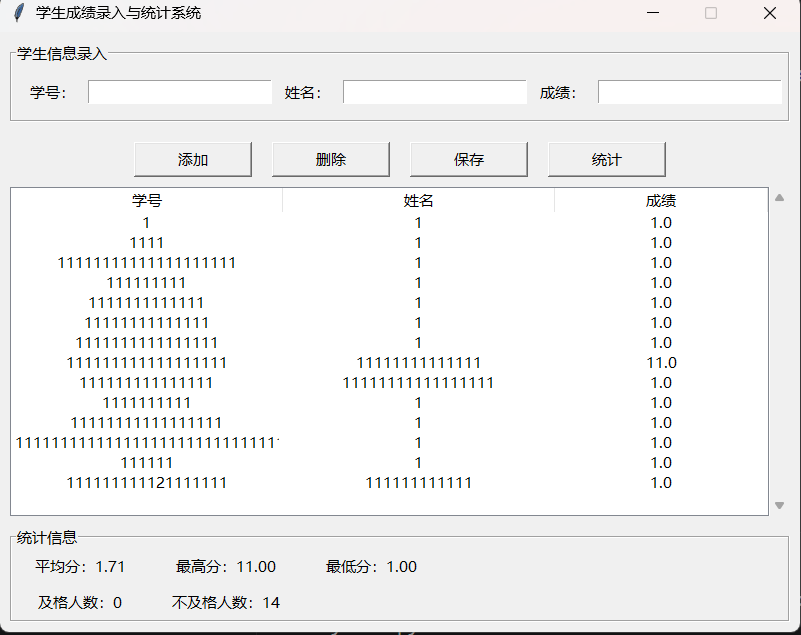
\includegraphics[width=\textwidth]{image.png}
    \caption{基于tkinter的学生成绩录入与统计系统的设计与实现}
    \label{fig:image}
\end{figure}
\subsubsection{基于opencv车牌识别系统}
代码：
\begin{verbatim}
class StudentScoreSystem:
"""
主函数
"""
def __init__(self):
    # 创建主窗口
    self.root = tk.Tk()
    self.root.title("学生成绩录入与统计系统")
    self.root.geometry("800x600")
    self.root.resizable(False, False)
    # 学生信息列表
    # 每个元素均为一个字典：
    # {"id": 学号, "name": 姓名, "score": 成绩}
    self.students = []
    # 创建图形界面
    self.create_widgets()
    # 读取历史保存的数据
    self.load_data()
    # 将数据刷新到TreeView中显示
    self.refresh_tree()

# 添加学生信息
def add_student(self):

    # 获取输入框中的内容，并去除首尾空格
    stu_id = self.entry_id.get().strip()
    name = self.entry_name.get().strip()
    score = self.entry_score.get().strip()

    # ---------- 输入合法性检查 ----------
    if stu_id == "":
        messagebox.showerror("输入错误", "学号不能为空！")
        return

    if name == "":
        messagebox.showerror("输入错误", "姓名不能为空！")
        return

    if score == "":
        messagebox.showerror("输入错误", "成绩不能为空！")
        return

    # 判断成绩是否为数字
    try:
        score = float(score)
    except ValueError:
        messagebox.showerror("输入错误", "成绩必须是数字！")
        return

    # 判断成绩是否在合法范围内
    if score < 0 or score > 100:
        messagebox.showerror("输入错误", "成绩必须在0~100之间！")
        return

    # 判断学号是否重复
    for stu in self.students:
        if stu["id"] == stu_id:
            messagebox.showerror("输入错误", "该学号已经存在！")
            return

    # ---------- 添加数据 ----------
    self.students.append(
        {
            "id": stu_id,
            "name": name,
            "score": score
        }
    )

    # 更新TreeView显示
    self.refresh_tree()

    # 清空输入框，方便继续录入
    self.entry_id.delete(0, tk.END)
    self.entry_name.delete(0, tk.END)
    self.entry_score.delete(0, tk.END)

    messagebox.showinfo("成功", "学生成绩添加成功！")

# 刷新TreeView中的数据
def refresh_tree(self):

    # 删除TreeView中已有数据
    for item in self.tree.get_children():
        self.tree.delete(item)

    # 将学生列表重新插入TreeView
    for stu in self.students:

        self.tree.insert(
            "",
            tk.END,
            values=(
                stu["id"],
                stu["name"],
                stu["score"]
            )
        )
# 保存学生成绩到CSV文件
def save_data(self):

    try:

        # 以写入方式打开CSV文件
        with open(
            "students.csv",
            "w",
            newline="",
            encoding="utf-8-sig"
        ) as file:

            writer = csv.writer(file)

            # 写入表头
            writer.writerow(
                ["学号", "姓名", "成绩"]
            )

            # 将学生数据逐行写入CSV文件
            for stu in self.students:

                writer.writerow(
                    [
                        stu["id"],
                        stu["name"],
                        stu["score"]
                    ]
                )

        messagebox.showinfo(
            "保存成功",
            "成绩数据已保存到 students.csv"
        )

    except Exception as e:

        # 保存失败时提示异常信息
        messagebox.showerror(
            "保存失败",
            str(e)
        )
\end{verbatim}

\subsection{小结}
本实验基于 OpenCV、Tkinter 和 pytesseract 实现了车牌识别系统，完成了图像读取、灰度化、图像预处理、车牌定位、字符识别以及结果显示等功能。通过实践掌握了数字图像处理的基本流程，加深了对图像分割、边缘检测、形态学处理及 OCR 技术的理解，同时提高了 Python 综合开发和调试能力。

\section{[题目2]实验四}
\subsection{1. 基于opencv车牌识别系统}
\subsubsection{实验目的}
针对静态车牌图像完成完整车牌识别流程开发。
借助 OpenCV 与 numpy 完 成图像灰度化、滤波去噪、边缘检测、形态学运算、轮廓筛选等图像预处理操作， 
定位图片内车牌区域并完成字符分割；
对分割后的字符进行特征匹配识别，
输出 车牌完整号码；
利用 tkinter 搭建简易可视化交互界面，
实现图片导入、图像处 理、识别结果实时展示功能，
搭建一套轻量化本地车牌图像识别工具，
掌握数字 图像处理与目标字符识别基础流程。 
实验数据： 各类含车牌静态图片，
包含不同光照、拍摄角度的车辆车牌图像作为识别
测试样本：https://tianchi.aliyun.com/dataset/203402。

\subsubsection{实验内容及要求}

\begin{enumerate}
    \item 开发语言与核心库限定：Python、numpy、opencv-python；
    \item 完成图像预处理、车牌定位、字符分割、字符识别整套图像处理算法 编写；
    \item 使用 tkinter 设计图形交互界面，支持本地车牌图片上传、原图显示、 处理中间效果图、最终识别结果展示；
    \item 程序模块化设计，图像预处理、车牌定位、字符识别、界面功能分开 封装，代码注释清晰可运行；
    \item 可加载本地车牌图片完成识别，界面直观输出识别到的车牌字符。
    
\end{enumerate}




\subsubsection{详细设计}
\paragraph{源代码（带注释）}
\subsubsection{基于opencv车牌识别系统}
代码：
\begin{verbatim}
# 增加学生
def add_student(self):

    # 获取输入内容
    stu_id = self.entry_id.get().strip()
    name = self.entry_name.get().strip()
    score = self.entry_score.get().strip()

    # 输入合法性检查
    if stu_id == "":
        messagebox.showerror("输入错误", "学号不能为空！")
        return

    if name == "":
        messagebox.showerror("输入错误", "姓名不能为空！")
        return

    if score == "":
        messagebox.showerror("输入错误", "成绩不能为空！")
        return

    # 成绩必须是数字
    try:
        score = float(score)
    except ValueError:
        messagebox.showerror("输入错误", "成绩必须是数字！")
        return

    # 成绩范围检查
    if score < 0 or score > 100:
        messagebox.showerror("输入错误", "成绩必须在0~100之间！")
        return

    # 学号不能重复
    for stu in self.students:
        if stu["id"] == stu_id:
            messagebox.showerror("输入错误", "该学号已经存在！")
            return

    # 添加学生信息
    self.students.append(
        {
            "id": stu_id,
            "name": name,
            "score": score
        }
    )

    # 刷新表格显示
    self.refresh_tree()

# 刷新TreeView中的数据
def refresh_tree(self):

    # 删除TreeView中的所有数据
    for item in self.tree.get_children():
        self.tree.delete(item)

    # 将学生列表重新显示到TreeView中
    for stu in self.students:

        self.tree.insert(
            "",
            tk.END,
            values=(
                stu["id"],
                stu["name"],
                stu["score"]
            )
        )

# 统计学生成绩信息
def statistics(self):

    # 判断是否存在学生数据
    if len(self.students) == 0:
        messagebox.showwarning(
            "提示",
            "暂无学生成绩数据！"
        )
        return

    # 提取所有成绩
    scores = []

    for stu in self.students:
        scores.append(stu["score"])

    # 计算平均分、最高分和最低分
    average = sum(scores) / len(scores)
    maximum = max(scores)
    minimum = min(scores)

    # 统计及格人数和不及格人数
    pass_num = 0
    fail_num = 0

    for score in scores:

        if score >= 60:
            pass_num += 1
        else:
            fail_num += 1

    # 更新统计信息显示
    self.label_avg.config(
        text=f"平均分：{average:.2f}"
    )

    self.label_max.config(
        text=f"最高分：{maximum:.2f}"
    )

    self.label_min.config(
        text=f"最低分：{minimum:.2f}"
    )

    self.label_pass.config(
        text=f"及格人数：{pass_num}"
    )

    self.label_fail.config(
        text=f"不及格人数：{fail_num}"
    )
\end{verbatim}

\subsection{实验中遇到的问题}
先前使用的代码：
\begin{verbatim}
    self.canvas = tk.Label(
    self.left_frame,
    width=640,
    height=480,
    relief=tk.SUNKEN,
    bg="white"
)
\end{verbatim}

修改之后的代码：
\begin{verbatim}
    self.canvas = tk.Canvas(
    self.left_frame,
    bg="white",
    relief=tk.SUNKEN
)
self.canvas.pack(fill=tk.BOTH, expand=True)
\end{verbatim}

\subsubsection{代码造成的影响}
会导致显示出来的页面空白
\subsubsection{原因分析}
\begin{enumerate}
    \item 误解了 Label 控件的 width 和 height 参数含义
在 Tkinter 中，Label 控件的 width 和 height 参数并不是以像素（Pixel）为单位，而是分别表示字符数和文本行数。
    \item 布局管理器无法合理分配空间
由于 Label 请求的显示区域过大，grid 布局管理器在计算窗口布局时无法合理分配空间，导致界面中的控件无法正常显示，最终表现为程序运行后窗口只有一片空白，而没有任何按钮和输入框。
    \item width 和 height 的取值虽然不合理，但并不是非法参数，因此 Tkinter不会产生异常，也不会进入 try...except 语句进行错误提示，导致程序表面上运行正常，但界面显示异常。
\end{enumerate}

\subsection{小结}
本实验利用 Tkinter 开发了学生成绩管理系统，实现了学生信息录入、删除、成绩统计以及 CSV 文件的保存与读取等功能。通过本实验熟悉了 Python 图形界面程序设计方法，掌握了事件驱动机制、数据管理及文件操作，进一步提高了综合运用 Python 完成小型管理系统开发的能力。

\section{[题目3]实验七}
\subsection{数据分析与可视化}
\subsubsection{实验目的}
\begin{enumerate}
    \item 熟悉 Python 标准库 csv 的用法。
    \item 熟悉 CSV 和 TXT 文件操作。
    \item 熟练安装扩展库 numpy、pandas、matplotlib。 
    \item 熟悉使用扩展库 pandas 进行数据分析的基本操作。 
    \item 熟悉使用扩展库 matplotlib 进行数据可视化的基本操作。
\end{enumerate}

\subsubsection{数据描述}
 利用 Python 模拟生成 2025 年某个饭店营业额的表格数据文件$$2025\_restaurant\_sales.csv$$，该饭店一年中有 300 天营业，
 营业时间不固定， 每日销售额在500到1500之间，并随机选择10\%
 比例的销售额设置为$$NaN$$。
\subsection{实验内容及要求}
\begin{enumerate}
    \item 使用tkinter 设计图形化界面，界面布局清晰，操作按钮完整。
    \item 每条成绩记录至少包含学号、姓名和成绩三个字段。
    \item 实现成绩信息的添加、删除、显示、保存和读取功能。
    \item 使用CSV文件保存成绩数据，程序关闭后再次运行时能够读取已有数据。
    \item 实现成绩统计功能，包括平均分、最高分、最低分、及格人数和不及格 人数。
    \item 进行必要的输入合法性检查，例如学号和姓名不能为空，成绩必须为0 到100之间的数字。
    \item 代码结构清晰，主要功能应封装为函数或类，并添加必要注释。
    \item 运行结果中应展示正常输入、错误输入、数据保存、数据读取和统计结 果等测试情况。
    
\end{enumerate}

\subsubsection{详细设计}

\paragraph{源代码（带注释）}

\begin{figure}[H]
    \centering
    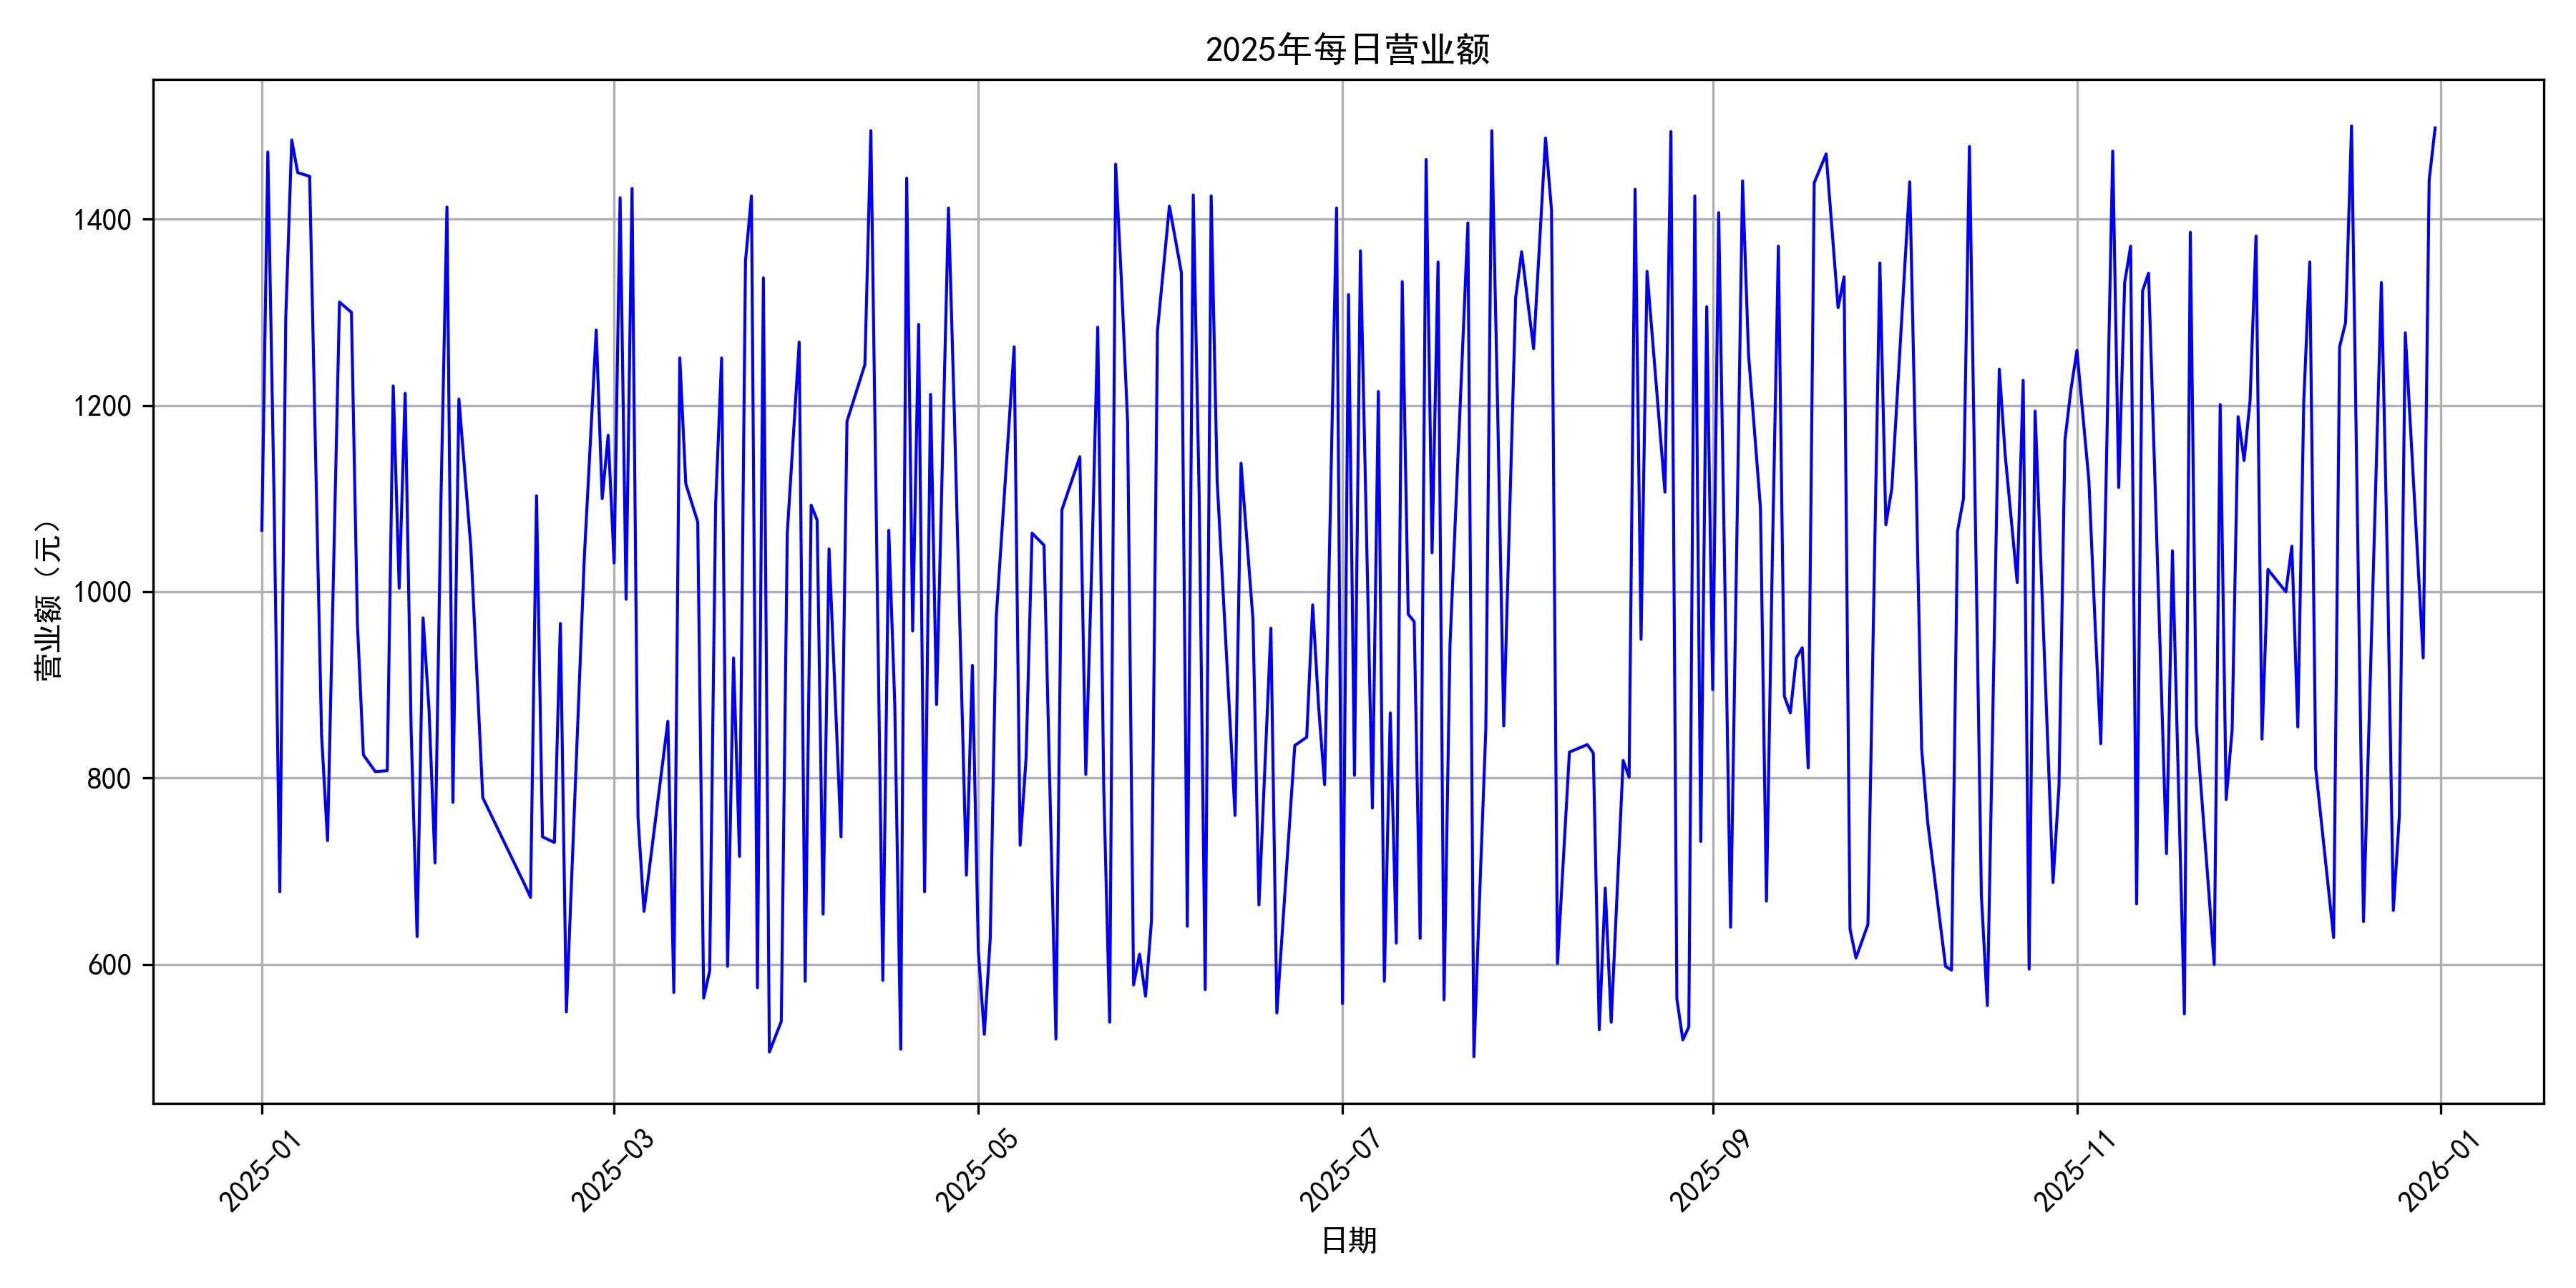
\includegraphics[width=\textwidth]{first.jpg}
    \caption{折线图}
    \label{fig:first}
\end{figure}

\begin{figure}[H]
    \centering
    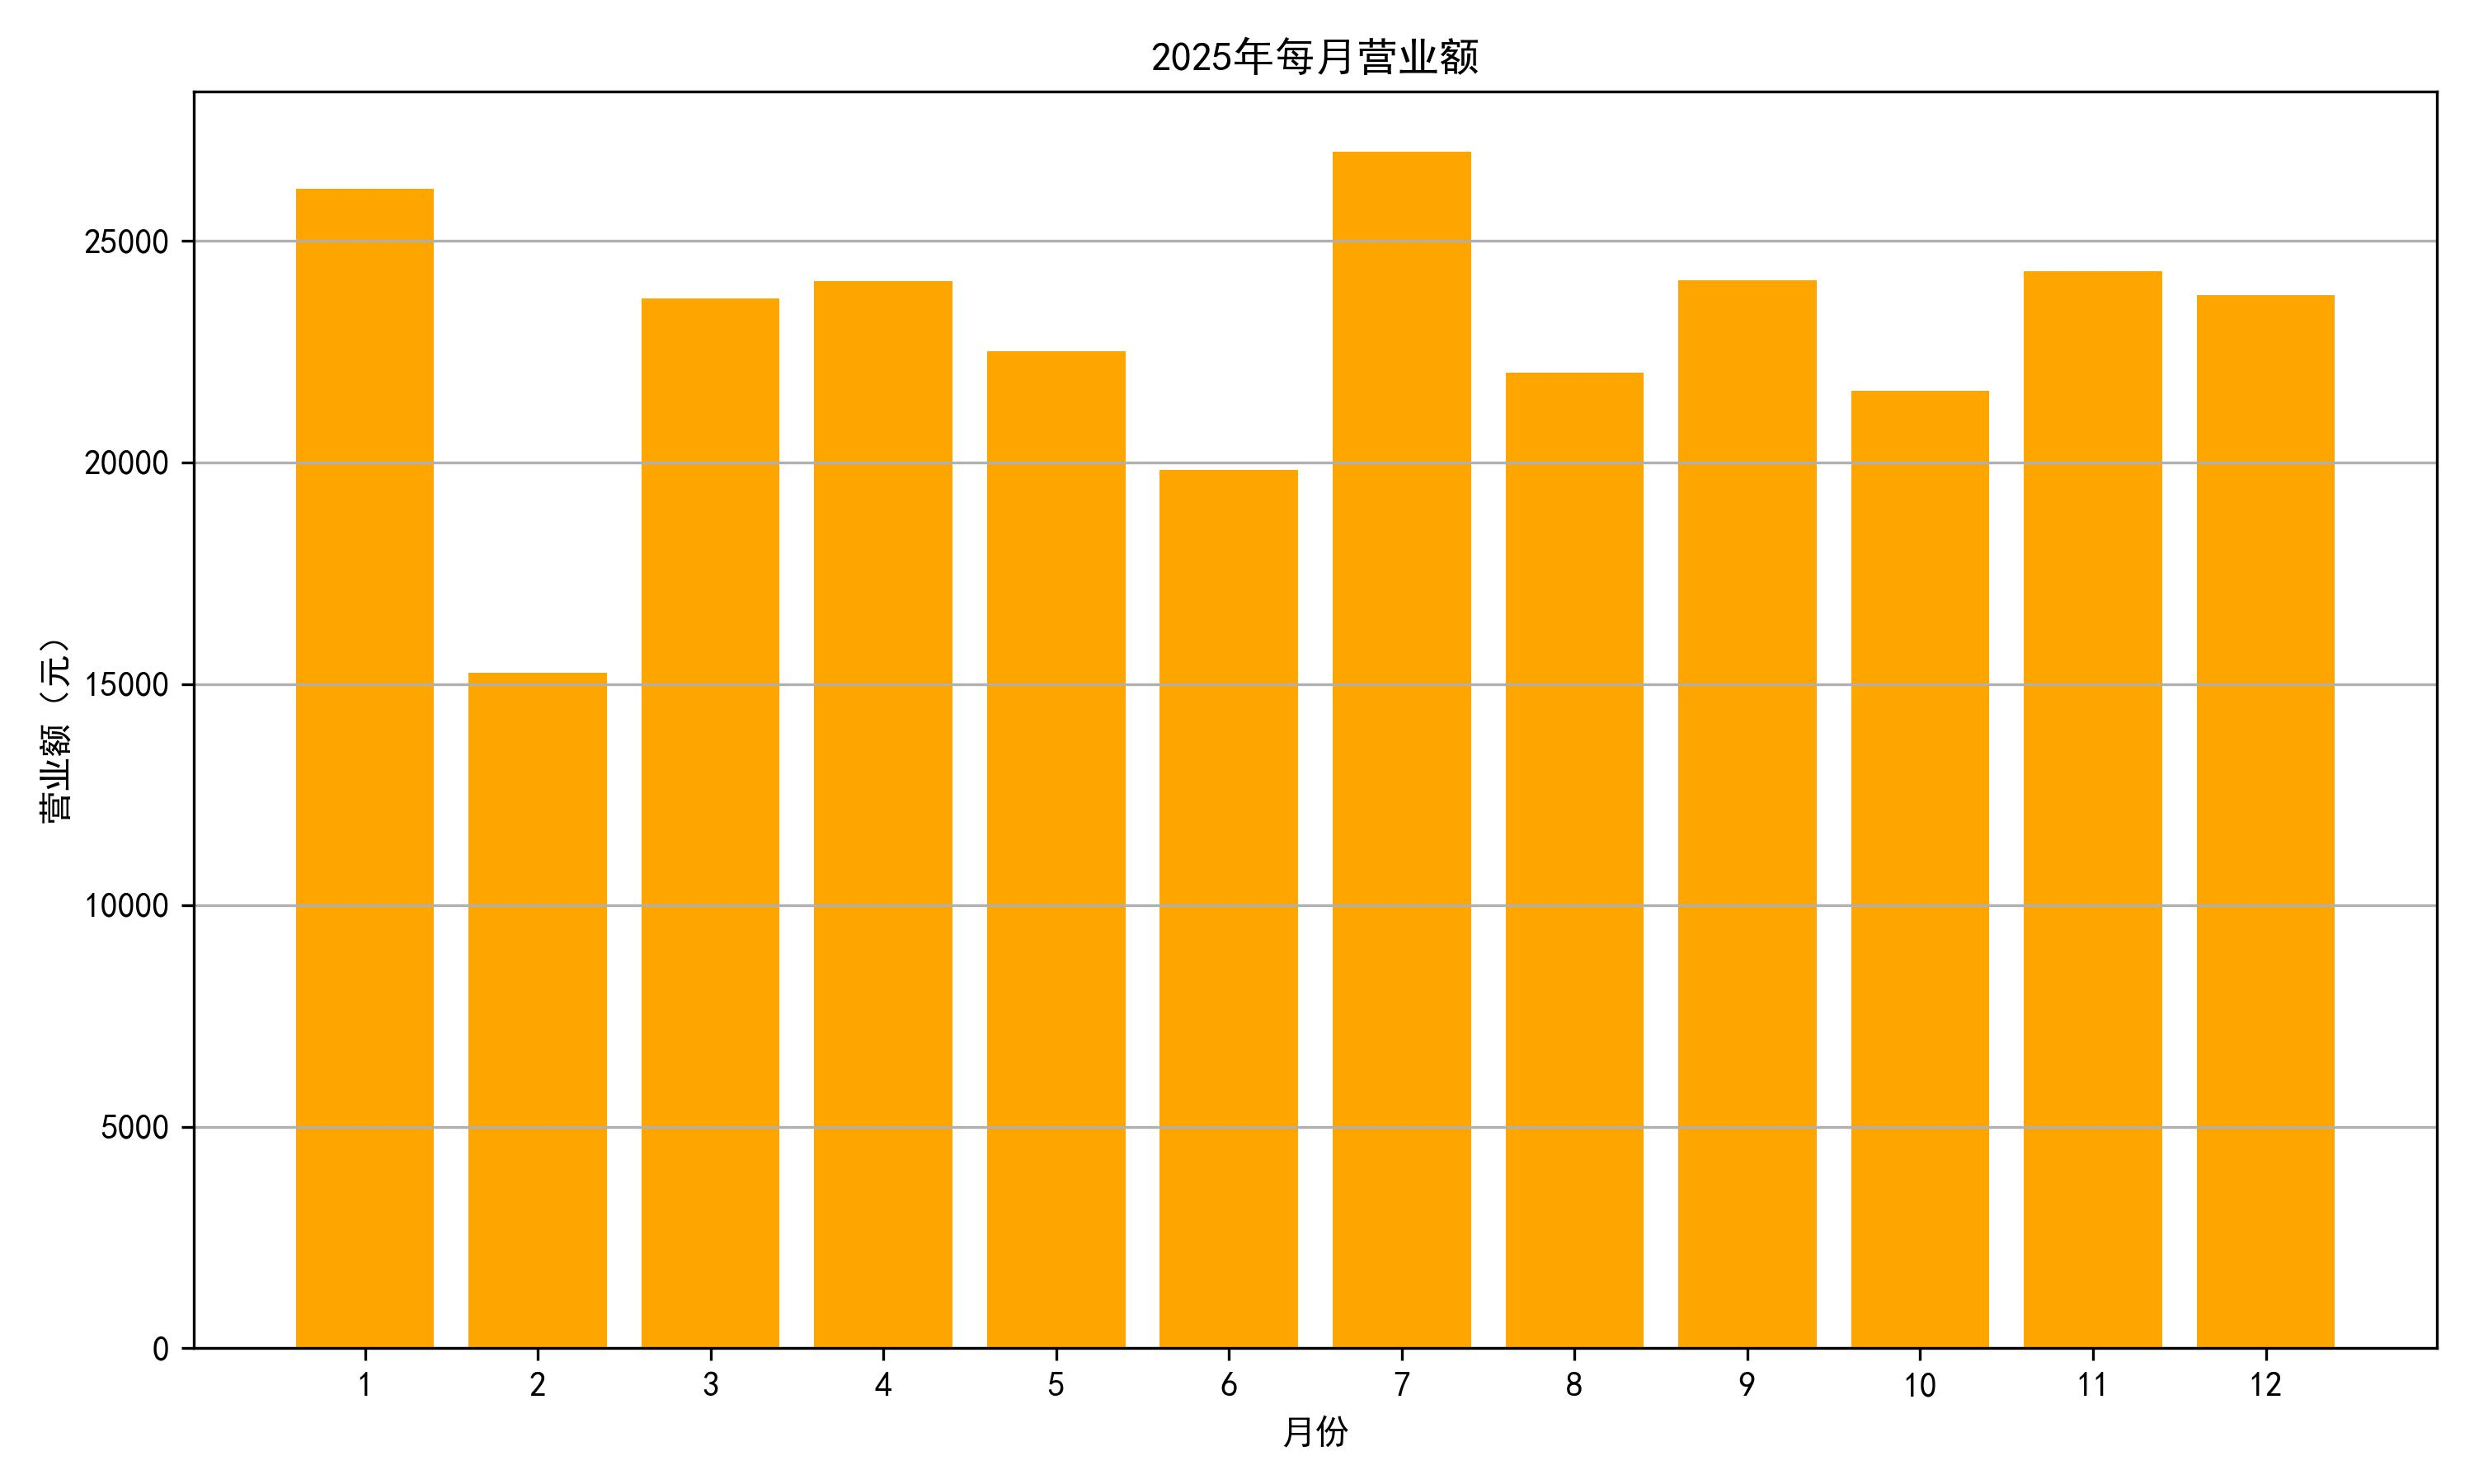
\includegraphics[width=\textwidth]{second.jpg}
    \caption{柱状图}
    \label{fig:second}
\end{figure}

\begin{figure}[H]
    \centering
    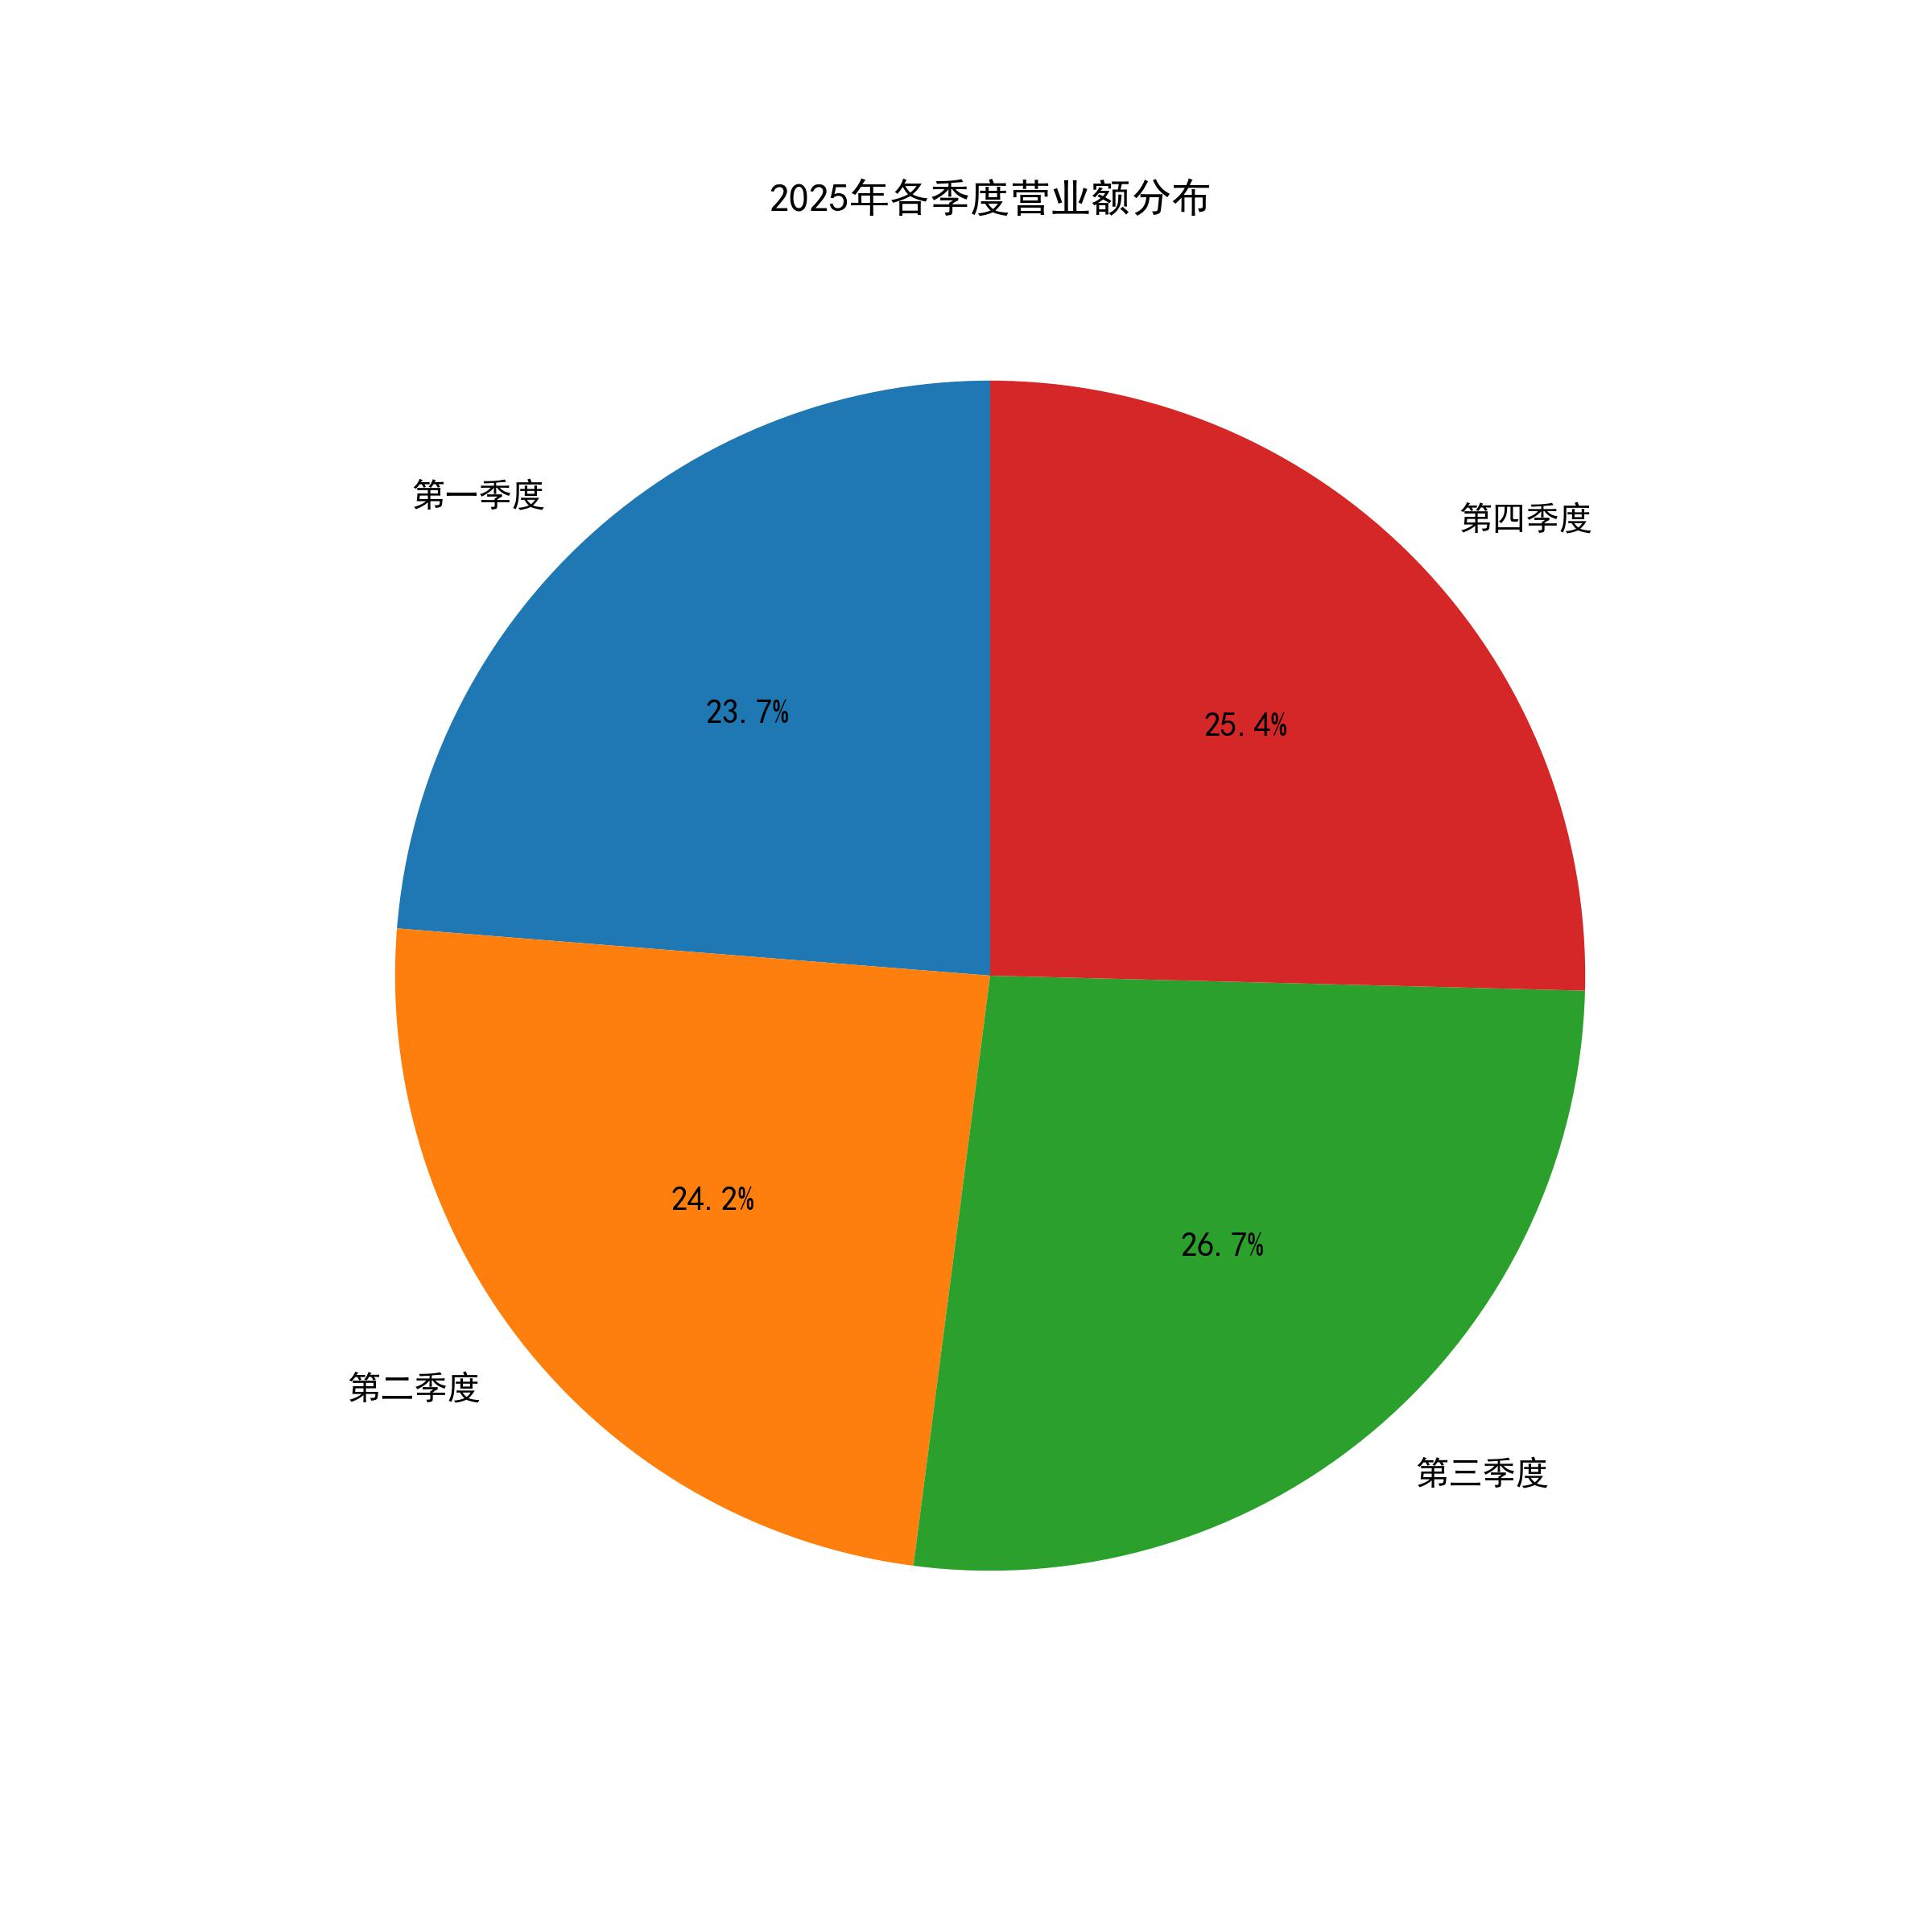
\includegraphics[width=\textwidth]{third.jpg}
    \caption{饼状图}
    \label{fig:thrid}
\end{figure}

\subsubsection{数据分析与可视化}
代码：
\begin{verbatim}
# 随机生成300天营业数据
for day in business_days:

    # 随机生成500~1500元营业额
    sales = random.randint(500, 1500)

    # 10%概率生成缺失值
    if random.random() < 0.1:
        sales = np.nan

    data.append([
        day.strftime("%Y-%m-%d"),
        sales
    ])

# 删除缺失值
def remove_nan(df):

    print(df.isnull().sum())

    # 删除所有缺失记录
    df = df.dropna()

    print(df.isnull().sum())

    return df

# 转换日期格式
df["Date"] = pd.to_datetime(df["Date"])

# 提取月份
df["Month"] = df["Date"].dt.month

# 按月份统计营业额
month_sales = df.groupby("Month")["Sales"].sum()

# 计算相邻月份营业额变化
growth = month_sales.diff()

# 找到最大涨幅月份
max_month = growth.idxmax()

max_growth = growth.max()

plt.figure(figsize=(12,6))

plt.plot(
    pd.to_datetime(df["Date"]),
    df["Sales"],
    linewidth=1
)

plt.title("2025年每日营业额")

plt.xlabel("日期")

plt.ylabel("营业额（元）")

plt.grid(True)

plt.savefig("first.jpg", dpi=300)
\end{verbatim}
\subsection{实验中遇到的问题}
\subsection{小结}
本实验采用 Pandas、NumPy 和 Matplotlib 完成了营业数据的生成、清洗、统计分析及可视化展示，实现了折线图、柱状图和饼图等多种图表绘制。通过实验掌握了数据预处理、分组统计和数据可视化的方法，加深了对 Python 数据分析流程的理解，为后续数据处理与分析应用奠定了基础。
\end{document}
